\part{Codifica di Canale}

\chapter{Teoria della Codifica di Canale}
Quanto analizzato per la codifica di sorgente ha senso esclusivamente nell'ipotesi in cui i dati non subiscano alterazioni durante la trasmissione. Tuttavia, i canali \textit{reali} sono \textbf{rumorosi} e possono introdurre errori in grado di degradare o distruggere il messaggio. La rimozione della ridondanza ottenuta tramite la codifica di sorgente, infatti, priva i dati di qualsiasi intrinseca robustezza: un errore nei metadati critici (come un albero di Huffman) o una \textit{desincronizzazione} nel flusso di bit può rendere l'intera sequenza incomprensibile a destinazione.

Per affrontare il problema di trasmettere in maniera affidabile su un canale non-affidabile, si ricorre alla \textbf{codifica di canale}, il cui limite teorico è governato dal \textbf{Secondo Teorema di Shannon}.

\section{Introduzione alla Codifica di Canale}
Mentre l'obiettivo della codifica di sorgente è ridurre la ridondanza per incrementare l'efficienza del sistema, l'approccio adottato nella codifica di canale è l'esatto opposto: introdurre ridondanza in modo strutturato per incrementare l'affidabilità.

L'algoritmo di codifica \textit{trasforma} la sequenza di dati in ingresso in una nuova sequenza di lunghezza maggiore, intrinsecamente più robusta agli effetti del rumore. Sfruttando questa ridondanza, in uscita dal canale, la decodifica di canale effettua l'operazione inversa: rileva l'eventuale presenza di errori e tenta di correggerli per ricostruire la sequenza di informazione originale prodotta dalla sorgente.

\begin{figure}[h]
    \centering
    \includesvg[width=1\linewidth]{img4/codifica_canale}
    \caption{Modello teorico del sistema di telecomunicazione}
    \label{fig:Modello teorico}
\end{figure}

Per semplicità, nel prosieguo della trattazione assumeremo che sia la sorgente, sia il canale di trasmissione siano discreti, tempo-invarianti e senza memoria. Su tali basi definiremo la quantità di informazione trasferita e la capacità del canale stesso.

\section{Modello Matematico del Canale Discreto}
Un canale di comunicazione \textbf{discreto} è caratterizzato da un alfabeto finito in ingresso (o sorgente) $X = \{x_1, x_2, \dots, x_K\}$ di cardinalità $K$, e un alfabeto finito in uscita (o destinazione) $Y = \{y_1, y_2, \dots, y_M\}$ di cardinalità $M$. Fenomeni \textit{rumorosi} o scelte progettuali possono far sì che l'alfabeto di destinazione differisca da quello in ingresso (ad esempio, possono verificarsi fenomeni di \textit{cancellazione}).

\begin{figure}[ht!] 
    \centering
    \includesvg[width=1\linewidth]{img4/canale_discreto}
    \caption{Modello del canale discreto}
    \label{fig:canale_discreto}
\end{figure}

\subsubsection{Notazione probabilistica}
Per descrivere statisticamente il comportamento del canale si definiscono le seguenti probabilità:
\begin{itemize}
    \item $P(x_i)$: probabilità \textit{a priori} che $x_i$ venga emesso dalla sorgente.
    \item $P(y_j)$: probabilità che $y_j$ venga ricevuto a destinazione.
    \item $P(x_i,y_j)$: probabilità \textbf{congiunta} che sia trasmesso $x_i$ e contemporaneamente ricevuto $y_j$.
    \item $P(x_i \mid y_j)$: probabilità \textbf{condizionata} (a posteriori) che sia stato trasmesso $x_i$ sapendo di aver ricevuto $y_j$.
    \item $P(y_j \mid x_i)$: probabilità \textbf{condizionata} (di transizione in avanti) che venga ricevuto $y_j$ data l'emissione di $x_i$.
\end{itemize}

\subsection{Canale discreto senza memoria tempo-invariante}
Nella nostra trattazione faremo riferimento a un modello di canale con due ipotesi semplificative fondamentali:
\begin{itemize}
    \item \textbf{Senza memoria:} l'uscita $y_j$ in un determinato istante $t$ dipende statisticamente \textbf{solo} dal simbolo in ingresso $x_i$ nello stesso istante $t$, ed è del tutto indipendente dai simboli trasmessi o ricevuti negli istanti precedenti.
    \item \textbf{Tempo-invariante (o stazionario):} le probabilità condizionate di transizione $P(y_j \mid x_i)$ non dipendono dall'istante di tempo in cui avviene la trasmissione, ma sono costanti nel tempo.
\end{itemize}
Un canale di questo tipo è \textbf{univocamente} definito dagli alfabeti $X$ e $Y$, e dall'insieme delle probabilità di transizione in avanti.

\begin{figure}[ht!] 
    \centering
    \includesvg[width=0.5\linewidth]{img4/prob_trans}
    \caption{Probabilità di transizione in avanti di un canale discreto con $K=2$ e $M=3$.}
    \label{fig:Prob transizione in avanti}
\end{figure}

\subsubsection{Matrice di transizione}
Essendo le probabilità di transizione stabilite e invarianti, possono essere organizzate in una matrice di dimensione $K \times M$, detta \textbf{matrice di transizione del canale} (o matrice canale):
\[
P = [P(y|x)] = \begin{bmatrix}
P(y_1|x_1) & P(y_2|x_1) & \dots & P(y_M|x_1) \\
P(y_1|x_2) & P(y_2|x_2) & \dots & P(y_M|x_2) \\
\vdots & \vdots & \ddots & \vdots \\
P(y_1|x_K) & P(y_2|x_K) & \dots & P(y_M|x_K)
\end{bmatrix}
\]
Trattandosi di probabilità condizionate, per la legge della probabilità totale, la somma degli elementi di ciascuna riga deve essere strettamente pari a $1$:
\[ \sum_{j=1}^M P(y_j|x_i) = 1 \quad \forall i = 1, \dots, K \]
\begin{figure}[htbp]
    \centering
    \[
    P =
    \begin{bmatrix}
        P(y_1 \mid x_1) & P(y_2 \mid x_2) & \dots  & P(y_K \mid x_1) \\
        P(y_1 \mid x_2) & \ddots &        &                 \\
        \vdots          &        & \ddots &                 \\
        P(y_1 \mid x_M) &        &        & P(y_K \mid x_M)
    \end{bmatrix}
    \]
    \caption{Matrice delle probabilità di transizione.}
    \label{fig:matrice_transizione}
\end{figure}



\section{Misure di Informazione e Capacità}
Per caratterizzare rigorosamente le prestazioni di un canale discreto e determinare i suoi limiti \textit{teorici} di trasmissione, è necessario estendere gli strumenti probabilistici introdotti per la sorgente al sistema congiunto ingresso-uscita.
Mentre l'entropia di sorgente $H(X)$ quantifica l'incertezza \textit{a priori} sul messaggio generato, ora l'attenzione è spostata sulla misura di come tale incertezza si modifichi a seguito dell'attraversamento del mezzo trasmissivo. Vogliamo cioè quantificare l'incertezza introdotta dal rumore e, per differenza, l'informazione utile che sopravvive alla trasmissione.
A tal fine, introduciamo nuove misure per l'entropia, che descrivono la relazione statistica tra la variabile aleatoria in ingresso a un canale, $X$, e quella di uscita $Y$.

\subsection{Entropie Condizionate: Rumore ed Equivocazione}
Alla ricezione di un particolare simbolo, essendo il canale \textit{rumoroso}, non abbiamo assoluta certezza su quale simbolo di $X$ in ingresso abbia portato a quel particolare $y$. L'evento \textit{ricezione di $y$} è un evento condizionato dall'evento \textbf{emissione di $x$}. Le probabilità sono descritte nella matrice di uscita - entrata e, in base a quei valori, possiamo calcolare l'\textbf{entropia condizionata per un particolare simbolo}:
\[H(X|y_j) = \sum_{x_i \in X}P(x_i|y_j)\log\left(\frac{1}{P(x_i|y_j)}\right)\]

$H(X|y_j)$ quantifica l'\textbf{incertezza sul simbolo trasmesso $x_i$ alla ricezione del simbolo $y_j$}. Il valore medio di $H(X|y_j)$ calcolato su tutti i possibili valori di $y_j$ identifica l'\textbf{equivocazione} (o entropia condizionata):
\[H(X|Y)=\sum_{j=1}^M H(X|y_j)P(y_j) = \sum_{j=1}^M \sum_{i=1}^K P(x_i,y_j)\log_2\left(\frac{1}{P(x_i|y_j)}\right) \]

Questa grandezza rappresenta l'incertezza residua \textbf{media} che permane sul simbolo trasmesso $X$, pur avendo osservato l'uscita $Y$. Nella Teoria dell'Informazione questo valore prende il nome di \textbf{Equivocazione}: misura la quantità di informazione che è andata perduta nel canale a causa del rumore e che, di conseguenza, non è giunta al destinatario. Si tratta, in sostanza, di un'incertezza \textit{a posteriori} rispetto alla ricezione dei simboli.

\paragraph{Ambiguità (o Entropia del Rumore)}
Esiste la quantità duale rispetto all'equivocazione, definita come $H(Y|X)$, che misura l'incertezza sull'uscita noto l'ingresso.
\[H(Y|X)=\sum_{x_i \in X}H(Y|x_i)P(x_i) = \sum_{x_i \in X}\sum_{y_j \in Y} P(x_i,y_j)\log\left(\frac{1}{P(y_j|x_i)}\right)\]

Questa grandezza è definita come la media delle entropie di riga della matrice di transizione, pesata con le probabilità della sorgente. Essa rappresenta quantitativamente il \textit{disordine} o \textit{rumore} introdotto dal canale.

\paragraph{Entropia Congiunta}
Infine, l'incertezza complessiva del sistema ingresso-uscita è descritta dall'Entropia Congiunta $H(X,Y)$. Essa misura l'informazione necessaria a descrivere contemporaneamente sia il simbolo trasmesso che quello ricevuto:
\[ H(X,Y) = \sum_{i=1}^{M} \sum_{j=1}^{K} P(x_i, y_j) \log\left(\frac{1}{P(x_i,y_j)}\right) \]

L'entropia del sistema globale corrisponde alla somma dell'entropia della sorgente ($H(X)$) e dell'ambiguità introdotta dal canale ($H(Y|X)$), o dualmente:
\[ H(X,Y) = H(X) + H(Y|X) = H(Y) + H(X|Y) \]


\subsection{Informazione Mutua}
Combinando le misure appena introdotte, arriviamo alla definizione di \textbf{Informazione Mutua} $I(X;Y)$.
Questa grandezza quantifica la riduzione di incertezza sulla sorgente $X$ ottenuta grazie all'osservazione dell'uscita $Y$.
Sfruttando le relazioni tra le entropie, l'informazione mutua può essere espressa in tre modi equivalenti:
\begin{enumerate}
\item \textbf{Differenza tra entropia di sorgente ed equivocazione:}
\[ I(X;Y) = H(X) - H(X|Y) \]
È la definizione base: l'informazione trasmessa è quella generata meno quella persa.

\item \textbf{Differenza tra entropia di uscita e ambiguità:}
\[ I(X;Y) = H(Y) - H(Y|X) \]
Utile per il calcolo della capacità, isola il rumore del canale.

\item \textbf{Relazione con l'entropia congiunta:}
\[ I(X;Y) = H(X) + H(Y) - H(X,Y)\]
Questa formula evidenzia che l'informazione mutua è la parte di informazione condivisa tra ingresso e uscita (la somma delle singole entropie sarebbe maggiore se fossero indipendenti).
\end{enumerate}

La quantità di informazione scambiata dal canale tra le variabili aleatorie $X$ e $Y$ è pari alle mutue informazioni delle stesse:
\[I(X;Y) = \sum_{i=1}^K \sum_{j=1}^M P(x_i,y_j) \log_2\left(\frac{P(x_i,y_j)}{P(x_i)P(y_j)}\right)\]
Utilizzando il teorema di Bayes $P(x_i,y_j) = P(x_i)P(y_j|x_i)$ a numeratore, e la probabilità totale a denominatore, si ottiene la forma esplicita in funzione della matrice di transizione e della sorgente:
\[I(X;Y) = \sum_{i=1}^K \sum_{j=1}^M P(x_i)P(y_j|x_i) \log_2 \left( \frac{P(y_j|x_i)}{\sum_{i=1}^K P(x_i)P(y_j|x_i)} \right)\]

\subsubsection{Proprietà dell'Informazione Mutua}
\begin{itemize}
    \item \textbf{Simmetria:}
        \[ I(X;Y) = I(Y;X) \]
        Anche se il canale fisico è direzionale (da $X$ a $Y$), la dipendenza statistica è reciproca: l'informazione che l'uscita fornisce sull'ingresso è quantitativamente identica a quella che l'ingresso fornisce sull'uscita.

    \item \textbf{Non negatività:}
        \[ I(X;Y) \geq 0 \]
        L'informazione mutua è sempre una quantità non negativa: osservare $Y$ nel peggiore dei casi lascia invariata l'incertezza su $X$, non può aumentarla.
    
    \item \textbf{Condizione di Indipendenza:}   
        La mutua informazione è nulla solo quando le due variabili risultano \textit{statisticamente indipendenti}; ciò avviene quando il rumore del canale impedisce totalmente il trasferimento di informazione.
\end{itemize}

\paragraph{Caso Ideale: Assenza di Rumore}
Consideriamo il caso limite, e ideale, di un canale privo di rumore. In assenza di disturbi, l'uscita del canale è \textbf{univocamente determinata} dall'ingresso. Ogni simbolo $y_j$ identifica uno ed un solo $x_i$:
\[ P(x_i \mid y_j) = 1 \Rightarrow I(x_i;y_j) = \log_2 \left( \frac{1}{P(x_i)}\right) = I_i \]
Conseguentemente, l'informazione veicolata dal canale coincide con l'autoinformazione del simbolo in ingresso. In media si ottiene il limite superiore:
\[I(X;Y)= H(X)\]

\paragraph{Caso Peggiore: Canale inutile (rumore infinito)}
Il caso limite opposto si ha quando il rumore è così elevato da rendere ingresso e uscita statisticamente indipendenti. Ricevere un simbolo $y_j$ non fornisce alcun contributo alla risoluzione dell'incertezza su $x_i$:
\[P(x_i \mid y_j) = P(x_i) \Rightarrow I(x_i;y_j) = \log_2 \left( \frac{P(x_i \mid y_j)}{P(x_i)} \right) = \log_2 1 = 0 \]
In questo caso, l'informazione mediamente trasferita è \textbf{nulla} ($I(X;Y) = 0$).

\section{Capacità di Canale}
Definiamo la \textbf{Capacità di Canale} $C_S$ come la misura delle prestazioni massime teoriche di un canale (\textit{discreto senza memoria}).
Matematicamente, si definisce come il \textbf{massimo} dell'informazione mutua, calcolabile variando le distribuzioni di probabilità in ingresso:
\[
C_S = \max_{\{P(x_i)\}} \{I(X;Y)\} \quad \left[ \frac{\text{bit}}{\text{simbolo}} \right]
\]
Espandendo l'informazione mutua utilizzando le misure di \textbf{equivocazione} e \textbf{ambiguità}, possiamo scrivere:
\[
C_S = \max_{\{P(x_i)\}} [H(X) - H(X|Y)] = \max_{\{P(x_i)\}} [H(Y) - H(Y|X)]
\]
Il valore di $C_S$ è \textit{indipendente dalla specifica sorgente}, poiché viene calcolato ipotizzando la distribuzione di probabilità in ingresso ottima, ovvero quella in grado di massimizzare il trasferimento di informazione. Di conseguenza, $C_S$ dipende unicamente dalla matrice di transizione (caratteristica intrinseca del canale), mentre l'Informazione Mutua $I(X;Y)$ è una misura che varia in funzione della specifica statistica della sorgente $X$ effettivamente utilizzata.

\paragraph{Capacità per unità di tempo}
Può essere utile esprimere la capacità del canale in termini di velocità di trasmissione. Se il sistema trasmissivo emette $r$ simboli al secondo (\textbf{symbol rate}), la capacità del canale per unità di tempo $C$ si ottiene moltiplicando la capacità per simbolo $C_S$ per la frequenza di simbolo:
\[ C = r \cdot C_S \quad \left[ \frac{\text{simboli}}{\text{sec}} \cdot \frac{\text{bit}}{\text{simbolo}} = \frac{\text{bit}}{\text{sec}} \right] \]

$C$ rappresenta la massima velocità teorica per il trasferimento di informazione consentita dal canale. In generale, il calcolo analitico della capacità non è banale; tuttavia, in caso di canale simmetrico, esso risulta notevolmente semplificato.

\paragraph{Esempio: calcolo capacità di canale simmetrico}
Consideriamo un canale con alfabeti in ingresso e uscita $X=Y=\{0,1,2,3,4\}$ e la seguente matrice di transizione:
\begin{center}
    \renewcommand{\arraystretch}{1.8} % Aumenta lo spazio verticale per le frazioni
    $P = \begin{bmatrix}
        0 & \frac{1}{2} & 0 & 0 & \frac{1}{2} \\
        \frac{1}{2} & 0 & \frac{1}{2} & 0 & 0 \\
        0 & \frac{1}{2} & 0 & \frac{1}{2} & 0 \\
        0 & 0 & \frac{1}{2} & 0 & \frac{1}{2} \\
        \frac{1}{2} & 0 & 0 & \frac{1}{2} & 0
    \end{bmatrix}$
\end{center}
Poiché le righe della matrice di transizione sono tutte permutazioni degli stessi valori, il canale è \textbf{simmetrico}. L'ambiguità introdotta dal canale (il termine $H(Y|X)$) dipende unicamente dai valori della riga ed è quindi una costante rispetto alla distribuzione in ingresso:
\[ H(Y|X) = H(Y|x_i) = -\left(\frac{1}{2}\log_2\frac{1}{2} + \frac{1}{2}\log_2\frac{1}{2}\right) = 1 \text{ bit} \]
La capacità di canale si ottiene massimizzando l'entropia dell'uscita $H(Y)$. Sappiamo che l'entropia massima per un alfabeto di $M=5$ simboli è $\log_2(5)$, e si ottiene quando l'uscita è equiprobabile. In un canale simmetrico, utilizzare un ingresso uniforme garantisce un'uscita altrettanto uniforme. Pertanto:
\[ C_S = \max_{\{P(x_i)\}}[H(Y)] - H(Y|X) = \log_2(5) - 1 \quad \left[\frac{\text{bit}}{\text{simbolo}}\right] \]
\section{Analisi di Canali Notevoli}
Analizziamo il comportamento dell'informazione mutua e della capacità per alcune tipologie specifiche di canali, classificati in base alla struttura della loro matrice di transizione.

\subsection{Canali Speciali (Classificazione Strutturale)}


\paragraph{Canale Senza Rumore (Ideale)}
% Matrice Identità. H(Y|X)=0. C = log M.
Questi canali sono caratterizzati dalla corrispondenza biunivoca tra ingresso e uscita.
%TODO: togliere commento
%\begin{center}
    % --- Minipage per l'equazione (Sinistra) ---
    \begin{minipage}{0.45\textwidth}
        \centering
        \[
        p(y_j \mid x_i) = 
        \begin{cases} 
            1 & \text{se } i = j \\ 
            0 & \text{se } i \neq j 
        \end{cases}
        \]
    \end{minipage}
    \hfill
    % --- Minipage per il grafico (Destra) ---
    \begin{minipage}{0.45\textwidth}
        \centering
        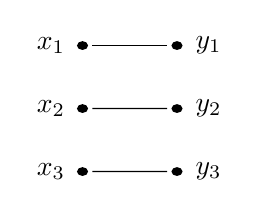
\begin{tikzpicture}[yscale=0.8]
            % Definizione dei nodi x e y con i punti
            \foreach \i in {1,2,3} {
                \node (x\i) at (0, -\i) {$x_\i$};
                \node (y\i) at (2, -\i) {$y_\i$};
                
                % Punti neri
                \fill (0.4, -\i) circle (2pt) node (dotx\i) {};
                \fill (1.6, -\i) circle (2pt) node (doty\i) {};
                
                % Linee di collegamento
                \draw (dotx\i) -- (doty\i);
            }
        \end{tikzpicture}
        
        \vspace{0.3cm}
        \small \textit{Esempio con $M=K=3$}
    \end{minipage}
\end{center}

\begin{itemize}
    \item La matrice di transizione è una \textbf{matrice identità}.
    \item Equivocazione e Ambiguità nulle: $H(X|Y) = H(Y|X) = 0 \Rightarrow I(X;Y) = H(X) = H(Y)$.
    \item $C_S = \max_{P(x)}\{I(X;Y)\} = \log_2(K)$ e si ottiene quando la distribuzione della sorgente $P(X)$ è \textbf{uniforme}.
\end{itemize}

\paragraph{Canale senza perdite}
In questo canale l'ingresso è totalmente determinato dall'uscita: l'osservazione del simbolo ricevuto elimina ogni incertezza su quale simbolo sia stato trasmesso. Matematicamente, questo si traduce in un'equivocazione nulla ($H(X|Y) = 0$). Nella matrice di transizione, ogni colonna contiene al massimo un solo elemento non nullo.
L'informazione mutua risulta $I(X;Y) = H(X)$, e la capacità è $C_S = \log_2(K)$.
%\begin{center}
    % --- Minipage Sinistra: Elenco puntato ---
    \begin{minipage}[c]{0.50\textwidth}
        \begin{itemize}
            \item $H(X|Y)=0$
            \item $C_S=\log(M)$ nel caso in cui $P$ sia \textbf{uniforme}
        \end{itemize}
    \end{minipage}
    \hfill
    % --- Minipage Destra: Grafico ---
    \begin{minipage}[c]{0.40\textwidth}
        \centering
        \begin{tikzpicture}[yscale=0.6, >=Stealth]
            \node (x1L) at (-0.6, -1) {$x_1$}; \fill (0, -1) circle (2.2pt) coordinate (x1);
            \node (x2L) at (-0.6, -2.5) {$x_2$}; \fill (0, -2.5) circle (2.2pt) coordinate (x2);
            \node (x3L) at (-0.6, -4) {$x_3$}; \fill (0, -4) circle (2.2pt) coordinate (x3);

            \fill (2, 0) circle (2.2pt) coordinate (y5); \node at (2.5, 0) {$y_5$};
            \fill (2, -1) circle (2.2pt) coordinate (y1); \node at (2.5, -1) {$y_1$};
            \fill (2, -2.5) circle (2.2pt) coordinate (y2); \node at (2.5, -2.5) {$y_2$};
            \fill (2, -4) circle (2.2pt) coordinate (y3); \node at (2.5, -4) {$y_3$};
            \fill (2, -5) circle (2.2pt) coordinate (y4); \node at (2.5, -5) {$y_4$};

            \draw[thin] (x1) -- (y5);
            \draw[thin] (x1) -- (y1);
            \draw[thin] (x2) -- (y2);
            \draw[thin] (x3) -- (y3);
            \draw[thin] (x3) -- (y4);
        \end{tikzpicture}
        \par\vspace{0.3cm} 
        \small \textit{Esempio con $M=5,K=3$}
    \end{minipage}
\end{center}


\paragraph{Canale Deterministico}
Un canale si definisce deterministico quando ogni simbolo in ingresso determina \textbf{univocamente} il simbolo in uscita. La matrice di transizione avrà un solo elemento pari a $1$ per riga, mentre tutti gli altri saranno pari a $0$.
Matematicamente questo implica un'ambiguità nulla:
\[ H(Y|X) = 0 \]
L'informazione mutua si riduce quindi alla sola entropia dell'uscita:
\[ I(X;Y) = H(Y) - H(Y|X) = H(Y) \]
La capacità del canale è data dal massimo dell'entropia dell'uscita, ovvero il logaritmo della cardinalità dell'alfabeto di uscita $M$:
\[ C_S = \max_{P(x)} \{ H(Y) \} = \log_2 M \quad [\text{bit/simbolo}] \]
Si tratta del caso \textit{speculare} al canale senza perdite: in questo caso non si crea incertezza \textit{nella trasmissione}.

\begin{center}
    % --- Minipage Sinistra: Equazione ---
    \begin{minipage}[c]{0.50\textwidth}
        \[
        p(y_j \mid x_i) = 
        \begin{cases} 
            1 & \text{se } i \in A_j \\ 
            0 & \text{se } i \notin A_j 
        \end{cases}
        \]
    \end{minipage}
    \hfill
    % --- Minipage Destra: Grafico con Didascalia ---
    \begin{minipage}[c]{0.45\textwidth}
        \centering
        \begin{tikzpicture}[yscale=0.75, xscale=1.2]
            % Colonna X (Ingressi da 1 a 5)
            \foreach \i in {1,2,3,4,5} {
                \node (xl\i) at (-0.5, -\i) {$x_\i$};
                \fill (0, -\i) circle (2.2pt) node (x\i) {};
            }

            % Colonna Y (Uscite da 1 a 3)
            \foreach \j in {1,2,3} {
                \fill (2, -\j) circle (2.2pt) node (y\j) {};
                \node at (2.5, -\j) {$y_\j$};
            }

            % Collegamenti
            \draw (x1) -- (y1);
            \draw (x2) -- (y2);
            \draw (x3) -- (y3);
            \draw (x4) -- (y3);
            \draw (x5) -- (y3);

            \node[draw=red, thick, inner sep=2pt, fit=(xl3) (x5), label=left:{\color{red}$A_3$}] {};
            
        \end{tikzpicture}
        
        \par\vspace{0.4cm}
        \small \textit{Esempio: $K=5,M=3;\space A_3 = \{x_3,x_4,x_5\}$}
    \end{minipage}
\end{center}

\textbf{Nota bene:} Il fatto che il canale sia deterministico non garantisce che sia senza perdite. Come si evince dalla definizione, se più ingressi "collassano" sullo stesso simbolo di uscita (funzione non iniettiva), si genera incertezza nel processo inverso. In tal caso l'equivocazione è \textbf{strettamente positiva} ($H(X|Y) > 0$), rendendo impossibile la perfetta ricostruzione dell'ingresso.



\paragraph{Canale Totalmente Rumoroso (Inutile)}
% Matrice con righe identiche. Uscita indipendente dall'ingresso. C = 0.
Quando il rumore in un canale è massimo, l'uscita sarà statisticamente indipendente dall'ingresso. La matrice di transizione sarà quindi costituita da righe identiche a segnalare che la probabilità di ricevere un certo simbolo $y$ è la stessa, indipendentemente da quale $x$ sia stato trasmesso:
\[ P(y_j|x_i) = P(y_j|x_k) \quad \forall i,k \]
In queste condizione un ricevitore non avrà alcuna possibilità di distinguere gli ingressi.
Matematicamente, l'indipendenza statistica ($P(y|x) = P(y)$) implica che l'osservazione dell'uscita non riduce l'incertezza sull'ingresso:
\[ H(X|Y) = H(X) \]
Di conseguenza, l'informazione mutua crolla a zero:
\[ I(X;Y) = H(X) - H(X|Y) = 0 \]
La capacità del canale è nulla ($C_S = 0$): il canale è di fatto "interrotto" e non permette alcun trasferimento di informazione.


\subsection{Canali Simmetrici e Uniformi}

Abbandoniamo i casi limite (ideali o degeneri) per analizzare una classe di canali che modella molte situazioni reali: i \textbf{canali simmetrici}.
Intuitivamente, quando il rumore incide negativamente su tutti i possibili simboli in ingresso in modo \textit{bilanciato} ed \textit{equo}, parliamo di canale \textbf{simmetrico}. 
Nessun simbolo di ingresso è "più protetto" o "più esposto" al rumore rispetto agli altri, e nessun simbolo di uscita tende ad apparire più spesso di altri a causa di distorsioni sistematiche del canale.
In altre parole, la struttura dell'errore è invariante rispetto al simbolo trasmesso.
 Nella matrice di transizione, questo si manifesterà con il fatto che ogni riga sarà una permutazione di ogni altra riga e conseguentemente, lo stesso accade per tutte le colonne.

%\begin{center}
    % --- Minipage Sinistra: Grafico ---
    \begin{minipage}[c]{0.55\textwidth}
        \centering
        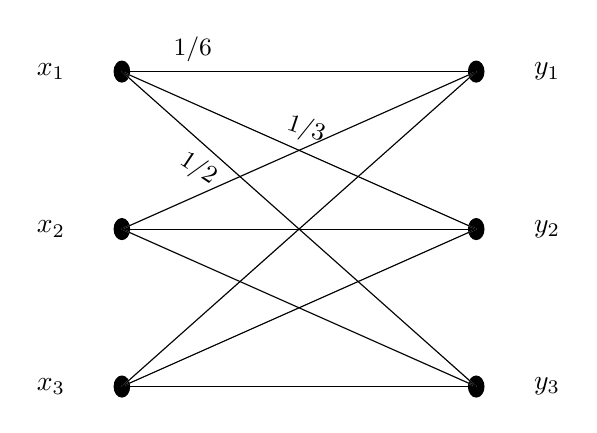
\begin{tikzpicture}[yscale=2.0, xscale=1.5] 
            % Nodi X e Y
            \foreach \i in {1,2,3} {
                \node (xl\i) at (-0.6, -\i) {$x_\i$};
                \fill (0, -\i) circle (2pt) coordinate (x\i);
                \fill (3, -\i) circle (2pt) coordinate (y\i);
                \node (yl\i) at (3.6, -\i) {$y_\i$};
            }

            % Rami di sfondo
            \foreach \i in {1,2,3} {
                \foreach \j in {1,2,3} {
                    \draw[thin, gray!30] (x\i) -- (y\j);
                }
            }

            % Rami x1 con etichette ancorate
            \draw[thin] (x1) -- node[above, pos=0.2] {\small 1/6} (y1);
            \draw[thin] (x1) -- node[above, pos=0.5, sloped] {\small 1/3} (y2);
            \draw[thin] (x1) -- node[below, pos=0.25, sloped] {\small 1/2} (y3);
            
            % Rami restanti neri
            \draw[thin] (x2) -- (y1); \draw[thin] (x2) -- (y2); \draw[thin] (x2) -- (y3);
            \draw[thin] (x3) -- (y1); \draw[thin] (x3) -- (y2); \draw[thin] (x3) -- (y3);
        \end{tikzpicture}
    \end{minipage}
    \hfill
    % --- Minipage Destra: Matrice ---
    \begin{minipage}[c]{0.40\textwidth}
        \centering
        % Dimensione standard per non farla sembrare piccola
        \normalsize 
        % Aumenta lo spazio tra le righe della matrice per matchare l'altezza del grafo
        \renewcommand{\arraystretch}{1.5} 
        \setlength{\arraycolsep}{6pt} 
        $\begin{pmatrix} 
            1/6 & 1/3 & 1/2 \\ 
            1/2 & 1/6 & 1/3 \\ 
            1/3 & 1/2 & 1/6 
        \end{pmatrix}$
        
        \par\vspace{0.3cm} % Spazio ridotto e armonizzato
        \small \textit{matrice di transizione}
    \end{minipage}
\end{center}


L'entropia condizionata $H(Y|x_i)$ è \textbf{indipendente} dal simbolo $x_i$, perché non dipende dalla riga della matrice di transizione usata per calcolarla.

\[H(Y|X)= \sum_{i=1}^Mp(x_i)H(Y|x_i)= H(Y|x_i) \quad \textit{Possiamo scegliere un qualsiasi $x_i$} \]

Per l'esempio precedente si ha che la capacità è:
\[C_S = \log_2(3) - H\left(\frac{1}{2},\frac{1}{3},\frac{1}{6}\right) = \frac{1}{2}\log_2(3) - \frac{2}{3}\]

\begin{align*}
H\left(\frac{1}{2}, \frac{1}{3}, \frac{1}{6}\right) &= - \left[ \frac{1}{2}\log_2\left(\frac{1}{2}\right) + \frac{1}{3}\log_2\left(\frac{1}{3}\right) + \frac{1}{6}\log_2\left(\frac{1}{6}\right) \right] \\
&= \frac{1}{2}\log_2 2 + \frac{1}{3}\log_2 3 + \frac{1}{6}\log_2 6 \\
&= \frac{1}{2}(1) + \frac{1}{3}\log_2 3 + \frac{1}{6}(\log_2 2 + \log_2 3) \\
&= \frac{1}{2} + \frac{1}{3}\log_2 3 + \frac{1}{6}(1 + \log_2 3) \\
&= \left( \frac{1}{2} + \frac{1}{6} \right) + \left( \frac{1}{3} + \frac{1}{6} \right)\log_2 3 \\
&= \frac{2}{3} + \frac{1}{2}\log_2 3
\end{align*}

Sostituendo questo risultato nella formula della capacità:
\begin{align*}
C &= \log_2 3 - \left( \frac{2}{3} + \frac{1}{2}\log_2 3 \right) \\
&= \log_2 3 - \frac{1}{2}\log_2 3 - \frac{2}{3} \\
&= \frac{1}{2}\log_2 3 - \frac{2}{3} \quad [\text{bit/simbolo}]
\end{align*}

Il termine $H(Y|x_i)$ rappresenta l'incertezza introdotta dal canale (rumore). Poiché in un canale simmetrico questo valore è costante per ogni riga, esso dipende esclusivamente dalle caratteristiche fisiche del canale e non dalla statistica della sorgente.

Per calcolare la capacità, dobbiamo massimizzare l'informazione mutua:
\[ C_S = \max_{P(X)} \{ H(Y) - H(Y|X) \} = \max_{P(X)} \{ H(Y) \} - H(Y|x_1) \]
Poiché il secondo termine è fisso, massimizzare la capacità equivale a massimizzare l'entropia di uscita $H(Y)$.
Sappiamo che l'entropia $H(Y)$ è massima quando la distribuzione di uscita è \textbf{uniforme} (tutti i simboli di uscita sono equiprobabili).
In un canale simmetrico, una distribuzione uniforme in ingresso genera una distribuzione uniforme in uscita.

Pertanto, la capacità si ottiene semplicemente sottraendo l'entropia di una riga al massimo valore teorico dell'entropia di uscita:
\[ C_S = \log_2 K - H(Y|x_1) \]
dove $K$ è il numero di simboli di uscita (cardinalità dell'alfabeto $Y$).


\subsection{Il Canale Binario Simmetrico (BSC)}
% Descrizione del modello (parametro p, input/output binari).
Il modello più importante di canale simmetrico è il \textbf{Canale Binario Simmetrico BSC} che modella la trasmissione di singoli bit su un canale rumoroso. È il caso più semplice di canale simmetrico.
Per definizione presenta queste caratteristiche:
\begin{itemize}
    \item alfabeto binario (simboli $x_1$ e $x_2$), caratterizzati da probabilità $P(x_1)= p$ e $P(x_2)= 1-p$
    \item anche l'alfabeto a destinazione è binario, con simboli $y_1$ e $y_2$
    \item le probabilità di transizione valgono:
    \[P(y_1\mid x_2) = P(y_2 \mid x_1) = \alpha\]
    \[P(y_1\mid x_1) = P(y_2 \mid x_2) = 1- \alpha\]
\end{itemize}

\paragraph{Canale BSC - esempio 1}
%\begin{center}
\begin{tikzpicture}[
    node distance = 1.2cm and 4cm,
    point/.style = {circle, fill, inner sep=1.8pt},
    blue_arr/.style = {blue, -{Stealth[scale=0.8]}, thin},
    red_arr/.style = {red, -{Stealth}, shorten >=5pt, shorten <=5pt},
    font=\large
]

    % --- 1. PROBABILITÀ E NODI DI INGRESSO ---
    \node (p1) at (-4, 1) {$P(x_1) = P_1 = p$};
    \node (p2) at (-4, -1) {$P(x_2) = P_2 = 1 - p$};

    \node (xl1) at (-0.6, 1) {$x_1$};
    \node[point] (x1) at (0, 1) {};
    
    \node (xl2) at (-0.6, -1) {$x_2$};
    \node[point] (x2) at (0, -1) {};

    % --- 2. NODI DI USCITA ---
    \node[point] (y1) at (4, 1) {};
    \node (yl1) at (4.6, 1) {$y_1$};
    
    \node[point] (y2) at (4, -1) {};
    \node (yl2) at (4.6, -1) {$y_2$};

    % --- 3. COLLEGAMENTI (Linee nere del canale) ---
    \draw (x1.center) -- (y1.center);
    \draw (x2.center) -- (y2.center);
    \draw (x1.center) -- (y2.center);
    \draw (x2.center) -- (y1.center);

    % --- 4. FRECCE ROSSE (Input) ---
    \draw[red_arr] (p1) -- (xl1);
    \draw[red_arr] (p2) -- (xl2);

    % --- 5. ANNOTAZIONI BLU (Probabilità di transizione) ---
    % Sopra x1 -> y1
    \draw[blue_arr] (1.5, 1.4) -- node[above, font=\small] {$1-\alpha$} (2.5, 1.4);
    
    % Sotto x2 -> y2
    \draw[blue_arr] (1.5, -1.4) -- node[below, font=\small] {$1-\alpha$} (2.5, -1.4);
    
    % Diagonale x1 -> y2 (freccia alpha)
    \begin{scope}[shift={(2.8,-0.35)}, rotate=-26]
        \draw[blue_arr] (0,0) -- node[right, font=\small] {$\alpha$} (0.8,0);
    \end{scope}
    
    % Diagonale x2 -> y1 (freccia alpha)
    \begin{scope}[shift={(2.5,0.1)}, rotate=26]
        \draw[blue_arr] (0,0) -- node[right, font=\small, pos=0.8] {$\alpha$} (0.8,0);
    \end{scope}

\end{tikzpicture}
\end{center}


La matrice di transizione risulta:
\[
P = \begin{bmatrix}
P(y_1/x_1) & P(y_2/x_1) \\
P(y_1/x_2) & P(y_2/x_2)
\end{bmatrix} =
\begin{bmatrix}
1-\alpha & \alpha \\
\alpha & 1-\alpha
\end{bmatrix}
\]


\paragraph{Canale BSC - esempio 2}
Vogliamo calcolare l'informazione mutua $I(X;Y) = H(Y) - H(Y|X)$.
Definiamo la funzione di entropia di sorgente binaria $\Omega(q)$ come
\[\Omega(q) = q\log_2\left(\frac{1}{q}\right) + (1 - q) \log_2 \left(\frac{1}{1-q}\right)\]
Da cui deriva che valgono le seguenti condizioni:
\begin{itemize}
    \item \[H(Y) = \Omega\left[P(y_1)\right] = \Omega(\alpha + p - 2\alpha p) \]
    \item \[H(Y|X)= \Omega(\alpha)\]
\end{itemize}


Questo perché:
\[P(y_1)= p(1-\alpha) + (1-p)\alpha = p - p\alpha + \alpha - p\alpha = \alpha + p - 2\alpha p\]
E calcolando l'ambiguità come $H(Y|X) = \sum_{i=1}^2 P(x_i)H(Y|x_i)$, sapendo che le righe della matrice contengono le probabilità $\alpha$ e $1-\alpha$, si ottiene l'incertezza introdotta dal canale:
\[H(Y|X) = \Omega(\alpha) = \alpha \log_2\left(\frac{1}{\alpha}\right) + (1-\alpha)\log_2\left(\frac{1}{1-\alpha}\right)\]

\subsubsection{Mutua informazione del canale BSC}
In un canale BSC l'informazione mutua sarà:
\[I(X;Y)= H(Y) - H(Y|X) = \Omega(\alpha + p - 2\alpha p) - \Omega(\alpha)\]

\begin{figure}[ht!]
    \centering
    \includesvg[width=0.5\linewidth]{img4/grafico-bsc}
    \caption{Per ogni $\alpha$, la curva di $I(X;Y)$ ha il massimo per simboli equiprobabili ($p=0.5$)}
    \label{fig:grafico-bsc}
\end{figure}
\FloatBarrier

\subsubsection{Capacità del Canale BSC}
La capacità del canale è data dal massimo dell'informazione mutua. Come illustrato nel grafico, la massimizzazione si ottiene per simboli di ingresso equiprobabili ($p = 0.5$).
In questo caso, l'entropia di uscita $H(Y)$ raggiunge il suo massimo teorico (essendo l'alfabeto binario, il massimo è $\log_2(2) = 1$).
\[C_S = \max_{P(X)} \{I(X;Y)\} = \log_2(2) - H(Y|x_i) = 1 - \Omega(\alpha)\]
Ovvero:
\[C_S = 1 - \left[ \alpha \log_2\left(\frac{1}{\alpha}\right) + (1-\alpha) \log_2\left(\frac{1}{1-\alpha}\right) \right] \quad [\text{bit/simbolo}]\]


\subsection{Canale simmetrico q-ario}
Possiamo considerare come estensione del canale binario simmetrico un canale con $q$ simboli.
\begin{itemize}
    \item $M = K = q$ (simmetria)
    \item La matrice di transizione:
        \[
\renewcommand{\arraystretch}{2} % Aumenta lo spazio verticale per le frazioni
\begin{pmatrix} 
    1 - \epsilon & \frac{\epsilon}{q-1} & \frac{\epsilon}{q-1} & \dots & \frac{\epsilon}{q-1} \\ 
    \frac{\epsilon}{q-1} & 1 - \epsilon & \frac{\epsilon}{q-1} & & \vdots \\ 
    \vdots & & & & \vdots \\ 
    \frac{\epsilon}{q-1} & \dots & & \dots & 1 - \epsilon 
\end{pmatrix}
\]
\item La capacità:
\[C_S = \log_2(q) - H(Y|x_1) = \log_2(q) + (1-\epsilon)\log_2(1-\epsilon) + \epsilon \log_2\left(\frac{\epsilon}{q-1}\right)\]
\end{itemize}
%TODO: togliere commento
%\begin{center}
\begin{tikzpicture}[scale=1.2, >=Stealth]
    % Assi
    \draw[->] (0,0) -- (6,0) node[below] {$\epsilon$};
    \draw[->] (0,0) -- (0,4.5) node[left] {C};

    % Curve (disegnata con una curva di Bézier per fedeltà visiva)
    % Punto iniziale (0, 3.5), punto di minimo (3.5, 0), punto finale (5, 1.2)
    \draw[thick] (0,3.5) .. controls (1.5,0.5) and (2.5,0) .. (3.5,0) 
                 .. controls (4,0) and (4.5,0.2) .. (5,1.2);

    % Etichette asse Y
    \fill (0,3.5) circle (1pt);
    \node[left] at (0,3.5) {$\log q$};

    % Etichette asse X e ticks
    % Tick 1/2
    \draw (2, -0.1) -- (2, 0.1);
    \node[below] at (2, -0.1) {$1/2$};
    
    % Tick (q-1)/q
    \draw (3.5, -0.1) -- (3.5, 0.1);
    \node[below right] at (3.5, 0) {$\frac{q-1}{q}$};
    
    % Tick 1 e linea tratteggiata
    \draw (5, -0.1) -- (5, 0.1);
    \node[below] at (5, -0.1) {$1$};
    \draw[dashed] (5,0) -- (5,1.2);
    \node[above right] at (5, 1.2) {$\log \frac{q}{q-1}$};

    % Freccia blu in basso
    \draw[<->, blue, thick] (0.1, -0.6) -- (3.4, -0.6);
\end{tikzpicture}
\end{center}
Essendo un canale \textit{simmetrico}, in caso di errore, il ricevitore può ricevere \textbf{uno qualsiasi} degli altri simboli con la stessa identica probabilità.

\subsection{Canale Simmetrico con cancellazione}
In un canale con \textit{cancellazione}, il rumore non causa l'inversione di un simbolo nell'altro, ma ne impedisce la corretta lettura. Il ricevitore è consapevole della perdita del dato, che viene quindi mappato in un \textit{terzo} simbolo dedicato alla cancellazione.
Conseguentemente, l'alfabeto di uscita avrà cardinalità maggiore di quello in ingresso ($K=M+1$). Nel caso binario, avremo in ingresso due simboli e in uscita tre.

%TODO: togliere commento
%\begin{center}
    % --- Minipage Sinistra: Matrice di Transizione ---
    \begin{minipage}[c]{0.45\textwidth}
        \centering
        \renewcommand{\arraystretch}{1.5} % Spazio verticale interno alla matrice
        $\begin{pmatrix} 
            1-\epsilon & 0 & \epsilon \\ 
            0 & 1-\epsilon & \epsilon 
        \end{pmatrix}$
    \end{minipage}
    \hfill
    % --- Minipage Destra: Diagramma del Canale ---
    \begin{minipage}[c]{0.45\textwidth}
        \centering
        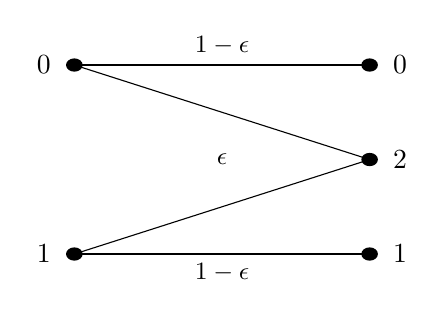
\begin{tikzpicture}[yscale=1.2, xscale=1.5]
            % Nodi di ingresso (Input: 0, 1)
            \node[left=5pt] at (0,0) {$0$}; \fill (0,0) circle (2pt) coordinate (x0);
            \node[left=5pt] at (0,-2) {$1$}; \fill (0,-2) circle (2pt) coordinate (x1);

            % Nodi di uscita (Output: 0, 2, 1)
            \fill (2.5,0) circle (2pt) coordinate (y0); \node[right=5pt] at (2.5,0) {$0$};
            \fill (2.5,-1) circle (2pt) coordinate (y2); \node[right=5pt] at (2.5,-1) {$2$};
            \fill (2.5,-2) circle (2pt) coordinate (y1); \node[right=5pt] at (2.5,-2) {$1$};

            % Collegamenti orizzontali (Successo)
            \draw (x0) -- node[above] {\small $1-\epsilon$} (y0);
            \draw (x1) -- node[below] {\small $1-\epsilon$} (y1);

            % Collegamenti diagonali verso l'uscita di cancellazione '2'
            \draw (x0) -- (y2);
            \draw (x1) -- (y2);
            
            % Etichetta epsilon centrale (Cancellazione)
            \node[fill=white, inner sep=2pt] at (1.25, -1) {\small $\epsilon$};
        \end{tikzpicture}
    \end{minipage}
\end{center}


\[H(Y|X) = \sum_{i=1}^M p(x_i)H(Y|x_i)= H(Y|x_1)= H(1-\epsilon,0,\epsilon) = H(1-\epsilon, \epsilon)\]
La capacità è data dalla formula:
\[C_S = \max_{P}\{H(Y)-H(Y|x_1)\} \quad \textbf{non dipende da $p$}\]

Essendo $H(Y|X)$ \textbf{costante} (pari a $H(1-\epsilon,\epsilon)$), bisogna massimizzare $H(Y)$.

La massimizzazione di $H(Y)$ si ottiene ponendo la probabilità di ingresso $p = 0.5$. Inserendo questo valore nello sviluppo dell'entropia di uscita, si ricava la capacità del canale con cancellazione:
\[ C_S = (1-\epsilon) \quad [\text{bit/simbolo}] \]
Questo risultato è intuitivo: una frazione $\epsilon$ dei bit viene cancellata (e non fornisce informazione), mentre la restante frazione $(1-\epsilon)$ arriva intatta (fornendo esattamente 1 bit di informazione ciascuno).

\subsection{Canale \textit{Z}}
In certe situazioni può accadere che in un canale binario i simboli $0$ vengano trasmessi senza errore, mentre i simboli $1$ siano affetti da una probabilità di errore che li porta ad essere erroneamente interpretati come $0$. Questo schema di errori asimmetrico è rilevante per modellare alcune situazioni, soprattutto in ambito di tecnologie di memorizzazione in cui i bit di valore $1$ hanno una probabilità di degradarsi col tempo, a differenza dei bit $0$.

Un canale binario \textit{Z} (con probabilità di errore $\frac{1}{2}$ come da esempio nelle slide) è definito nel seguente modo:

%\begin{center}
    % --- Minipage Sinistra: Matrice di Transizione ---
    \begin{minipage}[c]{0.40\textwidth}
        \centering
        \renewcommand{\arraystretch}{1.8} % Spazio verticale per le frazioni
        $P = \begin{bmatrix} 
            1 & 0 \\ 
            \frac{1}{2} & \frac{1}{2} 
        \end{bmatrix}$
    \end{minipage}
    \hfill
    % --- Minipage Destra: Diagramma del Canale ---
    \begin{minipage}[c]{0.50\textwidth}
        \centering
        \begin{tikzpicture}[yscale=1.5, xscale=2, >=Stealth]
            % Definizione nodi
            \node (x0) at (0, 1) {$0$};
            \node (x1) at (0, 0) {$1$};
            \node (y0) at (1.5, 1) {$0$};
            \node (y1) at (1.5, 0) {$1$};

            % Frecce blu con etichette
            \draw[->, blue, thick] (x0) -- node[above, black] {\small $1$} (y0);
            \draw[->, blue, thick] (x1) -- node[above, pos=0.6, black] {\small $\frac{1}{2}$} (y0);
            \draw[->, blue, thick] (x1) -- node[below, black] {\small $\frac{1}{2}$} (y1);
            
        \end{tikzpicture}
    \end{minipage}
\end{center}
\paragraph{Analisi e Capacità}
\begin{itemize}
    \item Alfabeti (simmetrici) $X=\{0,1\}$ e $Y=\{0,1\}$.
    \item \textbf{Uscita:} Se $p(x_1)= 1 - p$ e $p(x_2)= p$, le probabilità di uscita sono:
    \[ p(y_2) = p(y_2|x_2)p(x_2) = \frac{1}{2}p \]
    \[ p(y_1) = 1 - p(y_2) = 1 - \frac{p}{2} \]
    L'entropia di uscita risulta:
    \[ H(Y) = -\frac{p}{2}\log_2\left(\frac{p}{2}\right) - \left(1 -\frac{p}{2}\right)\log_2\left(1 -\frac{p}{2}\right) \]
    
    \item \textbf{Equivocazione:} Calcoliamo $H(Y|X)$. La prima riga (input 0) è deterministica ($H=0$), la seconda (input 1) ha entropia massima ($H=1$ bit).
    \[ H(Y|X) = p(x_1)\cdot 0 + p(x_2)\cdot 1 = p \]
    
    \item \textbf{Capacità:} Sostituendo nella formula dell'informazione mutua:
    \[ C_S = \max_P \{ H(Y) - H(Y|X) \} = \max_{0\leq p \leq 1} \{ H(Y) - p \} \]
    
    \item Il massimo della funzione si ottiene per $p = \frac{2}{5} = 0.4$, corrispondente a una capacità di:
    \[ C_S \approx 0.322 \text{ bit/simbolo} \]
\end{itemize}









